\documentclass{article}
\usepackage{amsmath}   % for mathematical equations
\usepackage{graphicx}  % for including graphs and images
\usepackage{float}     % to force figure placement
\usepackage{caption}   % for figure captions
\usepackage{siunitx}   % for units formatting
\usepackage{hyperref}  % for links

\title{Lab Report IV: Digital Logic}
\author{Enrique Rivera \\ Lab Partner: Marcus}
\date{\today}

\begin{document}
\maketitle

\section*{Lab 10: Digital Circuits I}

    \subsection*{Objective}
    The objective of Lab 10 was to familiarize students with basic logic gates and combinational circuits. The main focus was on building simple logic circuits using AND, OR, and NAND gates and verifying their truth tables through practical implementation.

    \subsection*{\textbf{Procedure - Question 1}}
    In this part of the lab, we used both TTL (7400N or 74LS00N) and CMOS (74HCT00N) ICs to implement individual logic gates. Each IC contains multiple NAND gates that can be configured into other basic gates (AND and OR) by connecting the gates in specific ways.

    \textbf{1. Power Supply Setup:}
    - We set the power supply (Vcc) to 5.04V, which is within the recommended operating range for both TTL and CMOS ICs.
    \\
    - Ground (GND) was connected to the ground terminal on the breadboard, and Vcc was applied to the power pins on the ICs.
    \\

    \textbf{2. Connecting the ICs:}
    - For each IC (TTL and CMOS), we connected Vcc (5.04V) to the designated power pin and ground to the ground pin of the ICs.
    \\
    - All unused inputs were grounded to prevent floating states, as floating inputs can lead to unpredictable behavior in CMOS and TTL logic gates.
    \\

    \textbf{3. Setting Up Inputs with SPDT Switches:}
    - We used SPDT (Single Pole Double Throw) switches on the breadboard to control the inputs for each gate. These switches allowed us to easily switch between 0 (ground) and 1 (Vcc) for each input, enabling us to test all possible input combinations.
    \\

    \textbf{4. Constructing NAND Gate Circuit:}
    - To test the NAND gate, we used one of the gates in the 7400N and 74HCT00N ICs. The input pins were connected to the SPDT switches for A and B, allowing us to manually control the input combinations (0 or 1).
    \\
    - LEDs were connected to the output pin through a current-limiting resistor to visualize the output. A high output (1) would turn the LED on, while a low output (0) would turn the LED off.
    \\

    \textbf{5. Testing Procedure:}
    - We applied all possible combinations of inputs (A and B) using the SPDT switches to observe the output.
    \\
    - For each combination, we recorded the LED state and documented whether the output matched the expected truth table values.
    \\

    \textbf{6. Verification with Multiple Gates:}
    - We repeated the procedure for additional gates on each IC to verify consistency in behavior. This was done by connecting different gate sections of the same IC, setting up inputs in a similar fashion, and observing the output with the same method.
    \\
    - We compared results between the TTL (7400N) and CMOS (74HCT00N) gates to observe any differences in behavior or performance.
    \\


    \subsection*{\textbf{Results - Question 1}}
    The following table and graph illustrate the expected truth table for the NAND gate tested in this question:

    \begin{table}[H]
        \centering
        \caption{Truth Table for NAND Gate}
        \begin{tabular}{|c|c|c|}
            \hline
            Input A & Input B & NAND Output \\
            \hline
            0 & 0 & 1 \\
            0 & 1 & 1 \\
            1 & 0 & 1 \\
            1 & 1 & 0 \\
            \hline
        \end{tabular}
    \end{table}

    \begin{figure}[H]
        \centering
        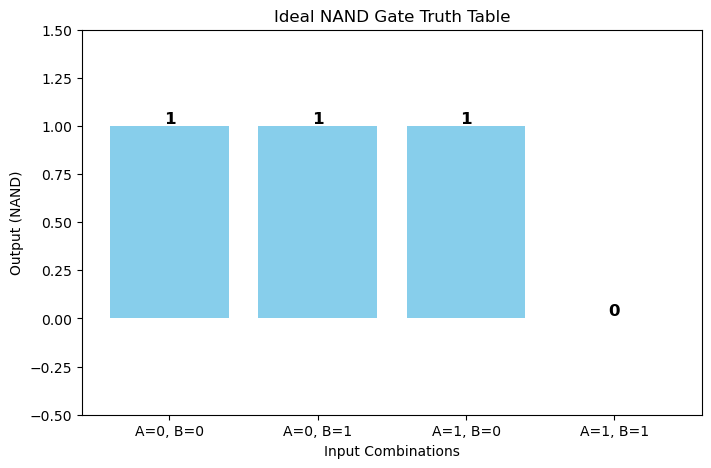
\includegraphics[width=0.7\textwidth]{./img/Lab 10/10_1_1.png}
        \caption{Ideal NAND Gate Truth Table Visualization}
        \label{fig:nand_truth_table}
    \end{figure}

    \subsection*{\textbf{Question 1 - Discussion}}
    The results confirmed that the NAND gate produces an output of 1 for all input combinations except when both inputs are 1, where it outputs 0. This behavior was consistent across both the TTL (7400N) and CMOS (74HCT00N) ICs, demonstrating their reliability in performing NAND operations. The truth table and visualization in Figure \ref{fig:nand_truth_table} match the theoretical expectations, validating the functionality of the NAND gates in our circuit. Additionally, grounding all unused inputs ensured stable outputs, particularly for the CMOS IC, which is more susceptible to interference from floating inputs. 
    \subsection*{\textbf{Procedure - Question 2}}
    In Question 2, we expanded the NAND gate circuit to implement a clocked flip-flop using two additional NAND gates. This configuration allowed us to create a clocked RS (Reset-Set) flip-flop, where the output changes state only when the clock is active.

    \textbf{1. Circuit Setup:}
   - We used the TTL (7400N) and CMOS (74HCT00N) ICs to build the flip-flop circuit.
   \\
   - Vcc was set to 5.04V, and all unused inputs were grounded to prevent floating states.
   \\
   - The circuit was connected so that two additional NAND gates were used to introduce a clock input, along with the S (Set) and R (Reset) inputs.
    \\

   \subsection*{\textbf{Procedure - Question 2}}
   In Question 2, we used multiple NAND gates to construct an \textbf{AND gate}. By configuring NAND gates in a specific arrangement, we replicated the behavior of a standard AND gate.

   \textbf{1. Circuit Setup:}
      - We used the TTL (7400N) and CMOS (74HCT00N) ICs, each containing multiple NAND gates.
      \\
      - Vcc was set to 5.04V, and all unused inputs were grounded to prevent floating states.
      \\
      - To create an AND gate using NAND gates, we connected two NAND gates in series:
      \\
        - The inputs (A and B) were connected to the first NAND gate.
        \\
        - The output of the first NAND gate was connected to both inputs of the second NAND gate (essentially inverting the output of the first NAND gate).
        \\
   
   \textbf{2. Input Control with SPDT Switches:}
      - SPDT switches on the breadboard were used to control the A and B inputs, allowing us to toggle each input between 0 (ground) and 1 (Vcc).
      \\
      - LEDs were used to indicate the output state.
      \\
   
   \textbf{3. Testing Procedure:}
      - We applied all possible combinations of A and B inputs using the SPDT switches and observed the output.
      \\
      - The output state was recorded for each combination to confirm that the NAND gate arrangement produced the expected AND gate behavior.
      \\
   
   \subsection*{\textbf{Results - Question 2}}
   The table below summarizes the expected truth table for the constructed AND gate:
   
   \begin{table}[H]
       \centering
       \caption{Truth Table for AND Gate Constructed with NAND Gates}
       \begin{tabular}{|c|c|c|}
           \hline
           Input A & Input B & AND Output \\
           \hline
           0 & 0 & 0 \\
           0 & 1 & 0 \\
           1 & 0 & 0 \\
           1 & 1 & 1 \\
           \hline
       \end{tabular}
   \end{table}

   \begin{figure}[H]
        \centering
        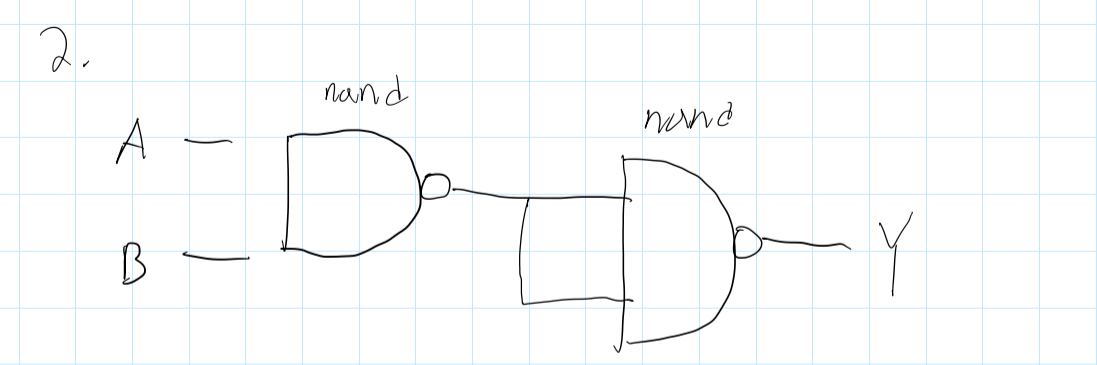
\includegraphics[width=0.7\textwidth]{./img/Lab 10/10_2_1.png}
        \caption{NANDS Gates to Construct AND Gate}
        \label{fig:and_gate}
    \end{figure}
   
   \subsection*{\textbf{Question 2 - Discussion}}
   The results confirmed that the arrangement of NAND gates successfully produced an AND gate. The output matched the expected truth table for an AND gate, outputting 1 only when both inputs were 1. This demonstrates that NAND gates can be used to create other basic gates, such as AND.
   
   \subsection*{\textbf{Procedure - Question 3}}
   In Question 3, we used multiple NAND gates to construct an \textbf{OR gate}. This required additional configuration, as NAND gates inherently perform a different operation.
   
   \textbf{1. Circuit Setup:}
      - We used the TTL (7400N) and CMOS (74HCT00N) ICs to build the OR gate circuit with NAND gates.
      \\
      - Vcc was set to 5.04V, and all unused inputs were grounded.
      \\
      - To create an OR gate using NAND gates, we used three NAND gates as follows:
      \\
        - The inputs A and B were each inverted by connecting them to separate NAND gates (where each input was connected to both pins of its NAND gate).
        \\
        - The outputs of these two NAND gates were then used as inputs to a third NAND gate.
        \\
   
   \textbf{2. Input Control with SPDT Switches:}
      - SPDT switches were used to control the inputs A and B, allowing us to switch each input between 0 and 1.
      \\
      - An LED was connected to the final output to visualize the OR gate's behavior.
      \\
   
   \textbf{3. Testing Procedure:}
      - We applied all possible combinations of A and B inputs using the SPDT switches and observed the output.
      \\
      - The output was recorded for each combination to confirm that the circuit configuration produced the expected OR gate behavior.
      \\
   
   \subsection*{\textbf{Results - Question 3}}
   The table below summarizes the expected truth table for the constructed OR gate:
   
   \begin{table}[H]
       \centering
       \caption{Truth Table for OR Gate Constructed with NAND Gates}
       \begin{tabular}{|c|c|c|}
           \hline
           Input A & Input B & OR Output \\
           \hline
           0 & 0 & 0 \\
           0 & 1 & 1 \\
           1 & 0 & 1 \\
           1 & 1 & 1 \\
           \hline
       \end{tabular}
   \end{table}

   \begin{figure}[H]
        \centering
        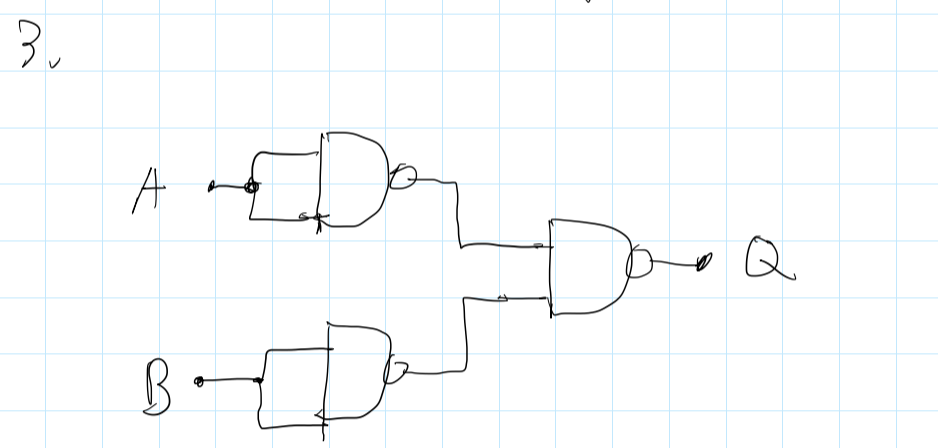
\includegraphics[width=0.7\textwidth]{./img/Lab 10/10_3_1.png}
        \caption{NANDS Gates to Construct OR Gate}
        \label{fig:or_gate}
    \end{figure}
   
   \subsection*{\textbf{Question 3 - Discussion}}
   The results confirmed that the configuration of NAND gates successfully produced an OR gate. The output followed the expected truth table for an OR gate, outputting 1 when either input was 1. This demonstrates that NAND gates can be used to create OR gates, providing flexibility in logic circuit design by combining basic components.
   
   \subsection*{\textbf{Procedure - Question 4}}
   For Question 4, we set up the CD4007 MOS transistor array, which contains six complementary MOS transistors (three N-channel and three P-channel FETs). This IC allowed us to configure the transistors to perform basic logic operations.
   
   \textbf{1. Component Identification:}
      - We identified the pins on the CD4007 corresponding to the N-channel and P-channel FETs, referring to Figure 2 in the lab manual for pin layout.
      \\
      - The N-channel FETs are used for low-side switching, and the P-channel FETs are used for high-side switching.
      \\
   
   \textbf{2. Setup:}
      - We configured the breadboard to prepare for the following exercises, ensuring that each transistor could be connected appropriately according to each circuit diagram.
      \\

    \subsection*{\textbf{Procedure - Question 5: Passive Pullup Inverter}}
    In Question 5, we built an inverter with a passive pullup resistor as shown in Figure 3.

    \begin{figure}[H]
        \centering
        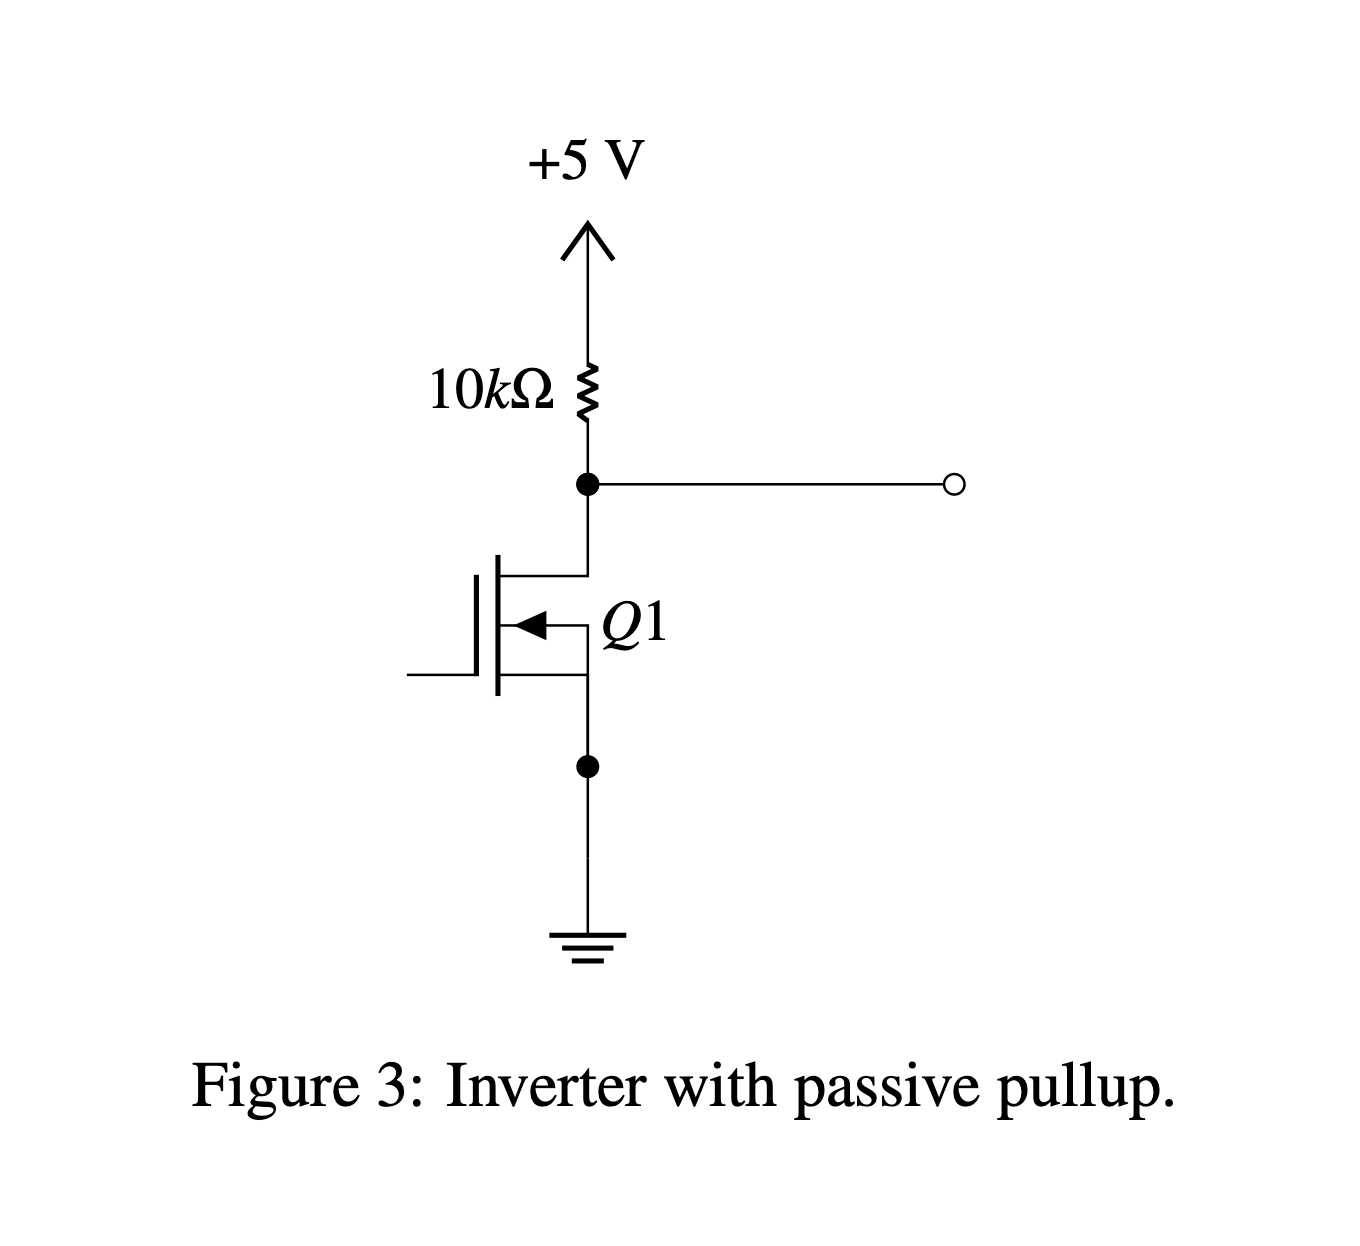
\includegraphics[width=0.7\textwidth]{./img/Lab 10/10_5_1.png}
        \caption{Passive Pullup Inverter Circuit}
        \label{fig:passive_pullup_inverter}
    \end{figure}

    \textbf{1. Circuit Construction:}
       - We connected the TTL output of the pulse generator to the input of the inverter.
       \\
       - A 1k resistor was used as a pullup, connecting the output to +5V.
       \\

    \textbf{2. Testing and Observations:}
       - We confirmed that the circuit inverted the input signal, outputting a low signal when the input was high and vice versa.
       \\
       - Next, we gradually increased the frequency of the input signal to determine the inverter’s behavior at higher frequencies.
       \\

    \subsection*{\textbf{Results - Question 5}}
    As we increased the frequency, we observed that the output started to degrade at high frequencies. The passive pullup could not fully charge or discharge the capacitance quickly enough, resulting in slower transitions and a less defined output.

    \subsection*{\textbf{Question 5 - Discussion}}
    The results indicate that while the passive pullup inverter performs adequately at lower frequencies, it suffers from significant degradation at higher frequencies. This is due to the time constant associated with the resistor and the inherent capacitance, which limits the circuit’s ability to respond to rapid changes in input.

    \subsection*{\textbf{Procedure - Question 6: Active Pullup Inverter}}
    In Question 6, we constructed an inverter using an active pullup configuration, as shown in Figure 4.

    \begin{figure}[H]
        \centering
        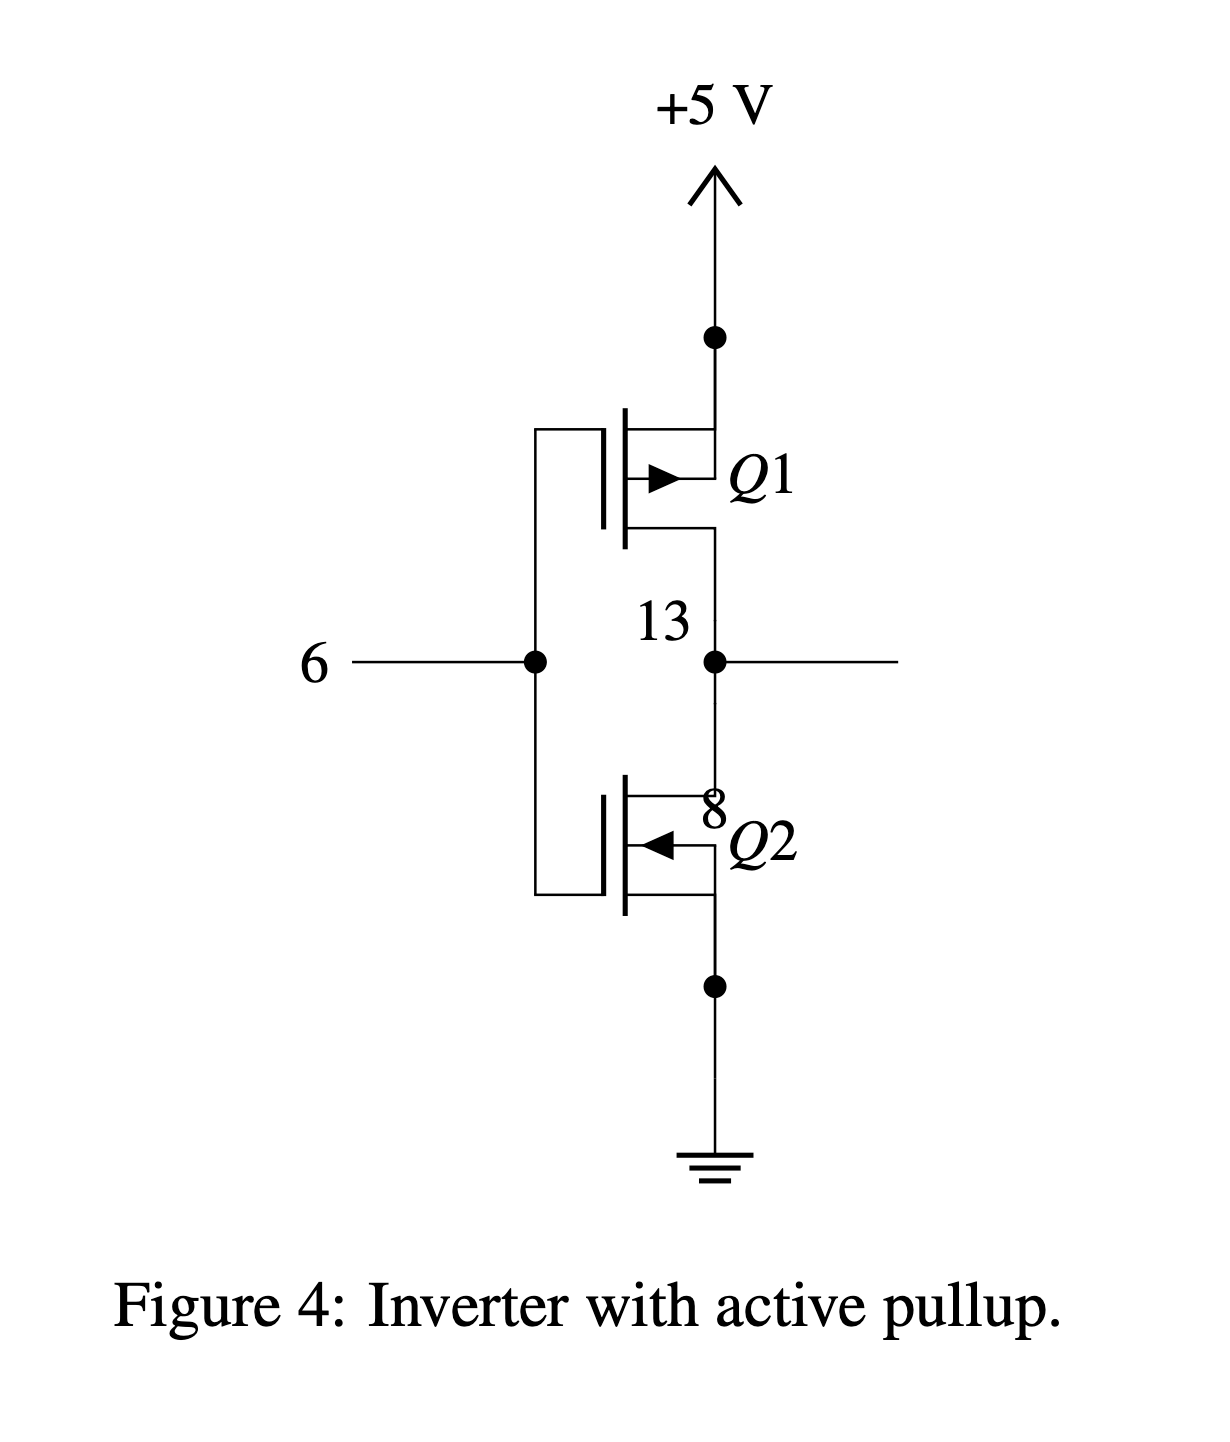
\includegraphics[width=0.7\textwidth]{./img/Lab 10/10_6_1.png}
        \caption{Passive Pullup Inverter Circuit}
        \label{fig:passive_pullup_inverter}
    \end{figure}

    \textbf{1. Circuit Construction:}
       - We used both an N-channel and a P-channel FET from the CD4007 to create an active pullup inverter.
       \\
       - The input signal was connected to both transistors, with the P-channel FET connected to +5V and the N-channel FET connected to ground.
       \\

    \textbf{2. Testing and Observations:}
       - We applied a TTL pulse from the generator to the input and observed the output on the oscilloscope.
       \\
       - As in the previous question, we increased the frequency of the input signal to observe any changes in behavior.
       \\

    \subsection*{\textbf{Results - Question 6}}
    The active pullup inverter demonstrated a more robust performance at higher frequencies compared to the passive pullup inverter. The output transitions were sharper and more consistent, with less signal degradation observed even as the input frequency increased significantly.

    \subsection*{\textbf{Question 6 - Discussion}}
    The active pullup inverter is more effective at handling high-frequency signals than the passive pullup configuration. The complementary configuration of N-channel and P-channel FETs allows for faster transitions, as each transistor actively pulls the output to the desired level, reducing the impact of capacitance.

    \subsection*{\textbf{Procedure - Question 7: NAND Gate Using CD4007 MOS Transistor Array}}
    In Question 7, we used the CD4007 MOS transistor array to construct a CMOS NAND gate using complementary MOSFETs. The CD4007 contains three N-channel and three P-channel MOSFETs, which can be configured to create various logic gates. We used two P-channel MOSFETs (for the pull-up network) and two N-channel MOSFETs (for the pull-down network) to form the NAND gate.
    
    \textbf{1. Pin Connections:}
    
    To replicate the CMOS NAND gate circuit, we used the following pin connections on the CD4007:
    
    \begin{itemize}
        \item \textbf{Vdd (Pin 14):} Connect this pin to the positive supply voltage (+5V). This supplies power to the P-channel MOSFETs.
        \item \textbf{GND (Pin 7):} Connect this pin to ground (0V), which serves as the ground for the N-channel MOSFETs.
        \item \textbf{Input A (Pin 6):} Connect this pin to the gate of both Q1 (P-channel) and Q3 (N-channel).
        \item \textbf{Input B (Pin 8):} Connect this pin to the gate of both Q2 (P-channel) and Q4 (N-channel).
        \item \textbf{Output (Pin 3):} This pin serves as the output of the NAND gate. It is the common connection between the drains of Q1 and Q2 (connected to Vdd) and the drains of Q3 and Q4 (connected to ground).
    \end{itemize}
    
    \begin{figure}[H]
        \centering
        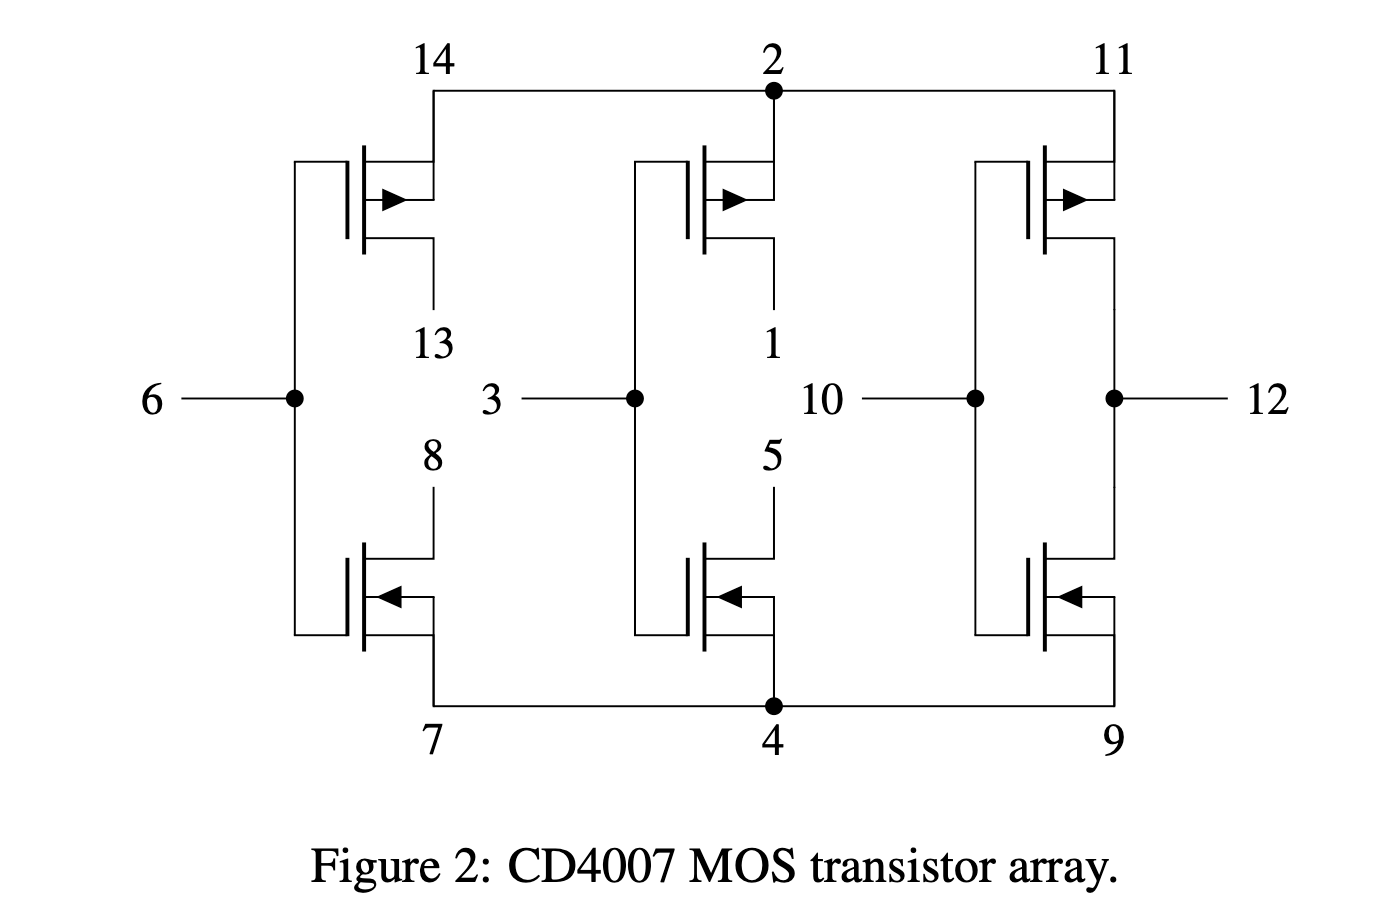
\includegraphics[width=0.5\textwidth]{./img/Lab 10/10_7_1.png}  % Replace with actual image path
        \caption{CMOS NAND Gate using CD4007 MOS Transistor Array}
        \label{fig:CMOS_NAND_Gate}
    \end{figure}
    
    \textbf{2. Operation of the CMOS NAND Gate:}
    
    The following describes the operation of the NAND gate based on the input combinations:
    
    \begin{itemize}
        \item \textbf{Input A = 0, Input B = 0:} Q1 and Q2 (P-channel MOSFETs) are \textbf{ON}, connecting the output to Vdd, resulting in a high output (1).
        \item \textbf{Input A = 0, Input B = 1:} Q1 remains \textbf{ON}, and Q4 is \textbf{OFF}, keeping the output high (1) through Q1.
        \item \textbf{Input A = 1, Input B = 0:} Q2 remains \textbf{ON}, and Q3 is \textbf{OFF}, keeping the output high (1) through Q2.
        \item \textbf{Input A = 1, Input B = 1:} Both Q1 and Q2 (P-channel MOSFETs) are \textbf{OFF}, while Q3 and Q4 (N-channel MOSFETs) are \textbf{ON}, creating a path to ground and resulting in a low output (0).
    \end{itemize}
    
    \subsection*{\textbf{Results - Question 7}}
    The truth table below summarizes the operation of the CMOS NAND gate circuit:
    
    \begin{table}[H]
        \centering
        \caption{Truth Table for CMOS NAND Gate}
        \begin{tabular}{|c|c|c|}
            \hline
            Input A & Input B & Output \\
            \hline
            0 & 0 & 1 \\
            0 & 1 & 1 \\
            1 & 0 & 1 \\
            1 & 1 & 0 \\
            \hline
        \end{tabular}
    \end{table}
    
    \subsection*{\textbf{Question 7 - Discussion}}
    The CMOS NAND gate operates as expected based on the complementary configuration of the transistors: \\ 
    
       - When both inputs are low (0), the P-channel transistors Q1 and Q2 conduct, pulling the output high.
       \\
       - If either input is low, at least one P-channel transistor is on, maintaining a high output.
       \\
       - When both inputs are high (1), the N-channel transistors Q3 and Q4 conduct, connecting the output to ground and resulting in a low output.
       \\
    
    This configuration leverages the complementary action of P-channel and N-channel MOSFETs, which allows for efficient switching with minimal power consumption when idle. CMOS technology provides good noise margins and low power dissipation, making it ideal for digital logic circuits. This experiment demonstrates that the CD4007 can be effectively used to create basic logic gates like the NAND gate.

\section*{Lab 11: Digital Circuits II}
  
\end{document}
